\documentclass[SE,authoryear,toc]{lsstdoc}
\usepackage{framed}
\definecolor{quoteleftbar}{rgb}{0.11,0.545,0.565}
\definecolor{quoteshade}{rgb}{0.95,0.995,0.995}
\definecolor{lightgrey}{RGB}{240, 240, 240}
% GENERATED FILE -- edit this in the Makefile
\newcommand{\lsstDocType}{SITCOMTN}
\newcommand{\lsstDocNum}{069}
\newcommand{\vcsRevision}{5236ac4-dirty}
\newcommand{\vcsDate}{2023-08-04}


% Package imports go here.
\usepackage[usestackEOL]{stackengine}

% Local commands go here.

%If you want glossaries
%\input{aglossary.tex}
%\makeglossaries

\title{LSB SciUnit Data Requirements Document}

% Optional subtitle
% \setDocSubtitle{A subtitle}

\author{
Lee S. Kelvin, Ian Dell'Antonio, Alex Drlica-Wagner, Annika Peter, Aaron Watkins, Yao-Yuan Mao, Amir E. Bazkiaei, Joshua~E.~Meyers
}

\setDocRef{SITCOMTN-069}
\setDocUpstreamLocation{\url{https://github.com/lsst-sitcom/sitcomtn-069}}

% The vcsDate command is not available without make;
% Commenting out here to allow Overleaf to compile.
\date{\vcsDate}

% Optional: name of the document's curator
% \setDocCurator{The Curator of this Document}

\setDocAbstract{%
This technote summarizes the data required by the Sky Background, Low Surface Brightness, Ghosts and Scattered Light SIT-Com Science Unit (LSB SciUnit) in order to begin testing our five identified normative requirements.
After analyzing each normative requirement, we conclude that required data falls into one of five categories: on-/off-axis bright star observations; pinhole camera data; collimated beam projector (CBP) data; full moon observations, and; galactic cirrus observations.
Of these categories, two do not necessarily require on-sky observations (pinhole camera data and CBP data), and one does not require high quality imaging (full moon observations).
It would be preferable for on-/off-axis bright star observations and observations of galactic cirrus to have higher quality imaging taken where possible, however, we anticipate the latter category to fall out during other observing campaigns, minimizing its impact on the planned schedule.
}

% Change history defined here.
% Order: oldest first.
% Fields: VERSION, DATE, DESCRIPTION, OWNER NAME.
% See LPM-51 for version number policy.
\setDocChangeRecord{%
  \addtohist{1}{2023-08-04}{Initial draft.}{Lee Kelvin}
}

% Custom myquote boxes to identify quoted text.
\newenvironment{myquote}[1][\hsize]
{
\def\FrameCommand
{
    {\color{quoteleftbar}\vrule width 3pt}%
    \fboxsep=\FrameSep\colorbox{quoteshade}%
}
\vspace{-0.25cm}
\MakeFramed{\hsize#1\advance\hsize-\width\FrameRestore}%
}
{\endMakeFramed\vspace{-0.75cm}}

\begin{document}

% Create the title page.
\maketitle
% Frequently for a technote we do not want a title page
% uncomment this to remove the title page and changelog.
% use \mkshorttitle to remove the extra pages

% ADD CONTENT HERE
% You can also use the \input command to include several content files.

\section{Introduction}  \label{sec:introduction}

The Sky Background, Low Surface Brightness, Ghosts and Scattered Light SIT-Com Science Unit (\textit{LSB SciUnit} hereafter) consists of in-kind contributor groups and associated interested parties concerned with matters relating to low surface brightness science.
See \href{https://sitcomtn-050.lsst.io/}{SITCOMTN-050} for a summary of the groups and individuals making in-kind contributions to the Vera C. Rubin Observatory System Integration, Test, and Commissioning (SIT-Com) effort.

The LSB SciUnit is charged with refining, verifying and validating five normative requirements taken from two key documents: \href{https://docushare.lsst.org/docushare/dsweb/Get/LSE-29}{LSE-29: LSST System Requirements (LSR)}, and \href{https://docushare.lsst.org/docushare/dsweb/Get/LSE-30}{LSE-30: Observatory System Specifications (OSS)}:
\begin{description}
  \item[Refine] \hfill \\ Analyze the normative requirements to determine the questions that need to be asked and the data required to address these questions.
  \item[Verify] \hfill \\ Check that the requirements are satisfied.
  \item[Validate] \hfill \\ Show that science can be done with these data products.
\end{description}

The purpose of this Data Requirements Document (\textit{DRD} hereafter) is to begin the first phase of this process, refining the initial definitions laid out in the two definition documents to precisely determine the questions we wish to ask and the data required to address those questions.

For more information, see the notes and linked resources listed on our \href{https://ls.st/sciunit-lsb}{LSB SciUnit Confluence page}.

\newpage





\section{Normative Requirements}  \label{sec:requirements}

The five normative requirements to be addressed under the remit of the LSB SciUnit are listed in the following table:

\addtocounter{table}{-1}
\begin{longtable}{p{0.17\textwidth}p{0.55\textwidth}p{0.23\textwidth}}\hline
\textbf{Requirement} & \textbf{Description} & \textbf{Focus Group}  \\\hline
\href{https://docushare.lsst.org/docushare/dsweb/Get/LSE-29\#page=29}{LSR-REQ-0009} & Stray and Scattered Light & \Centerstack[l]{Alex Drlica-Wagner \\ Ian Dell'Antonio} \\
\rowcolor{lightgrey}\href{https://docushare.lsst.org/docushare/dsweb/Get/LSE-30\#page=169}{OSS-REQ-0222} & Ghost Image Control & Lee Kelvin \\
\href{https://docushare.lsst.org/docushare/dsweb/Get/LSE-30\#page=170}{OSS-REQ-0223} & Lens Anti-Reflection Coating & \Centerstack[l]{Annika Peter \\ Lee Kelvin} \\
\rowcolor{lightgrey}\href{https://docushare.lsst.org/docushare/dsweb/Get/LSE-30\#page=171}{OSS-REQ-0225} & Lunar Stray Light & Ian Dell'Antonio \\
\href{https://docushare.lsst.org/docushare/dsweb/Get/LSE-30\#page=124}{OSS-REQ-0387} & Photometric Performance (ghosts, sky brightness) & \Centerstack[l]{Aaron Watkins \\ Yao-Yuan Mao \\ Amir E. Bazkiaei} \\\hline
\end{longtable}

The subsections below provide more detail on each requirement.
Our refined interpretation of the initial definition is presented, and the required data is described.

\newpage





\subsection{LSR-REQ-0009: Stray and Scattered Light}  \label{sec:stray}

\textbf{Focus Team:} Alex Drlica-Wagner, Ian Dell'Antonio

\begin{myquote}

\textbf{Requirement:} The LSST design shall control the effects of stray and scattered light to the extent necessary to meet the performance in the Survey Specifications.

\textbf{Discussion:} Discussion: Stray and scattered light is defined as any light that is not part of the ideal image and includes:
\begin{itemize}
    \item diffuse scattered light,
    \item secondary ghost images,
    \item diffraction, and
    \item structured glints.
\end{itemize}

\end{myquote}

\textbf{Analysis:} Stray and scattered light is defined as light that is not part of the ideal image and is not expected from the baseline optical model.
This is in contrast to "Ghosts" (Section \ref{sec:ghosts} and \ref{sec:arcoating}), which are the result of expected and unavoidable internal reflections. 
Stray and scattered light is generally expected to have the largest impact when it originates from bright sources (i.e., bright stars, the moon, or a light source internal to the dome).
There are many terms used for different aspects of stray and scattered light (e.g., ghouls, glints, sprays, etc.), which have historically corresponded to different production mechanisms (e.g., scattering off of surfaces in the filter changer, reflective surfaces within the camera, or reflections from camera elements that are difficult to include in the optical model).
See for example \citet{Kent2013} for a discussion of scattered light in DECam.

The primary goal of investigations into stray and scattered light is to cover a wide range of observational configurations in order to identify excess contributions of such light.
In particular, the data requirements are similar to those for Ghosts (i.e., targeting bright stars), but covering a wider range of configurations and orientations.
It may be the case that individual contributors to stray and scattered light may be identified and either corrected or incorporated into the optical model.
Machine learning methods have been demonstrated to be powerful tools for identifying stray and scattered light in images \citep{Chang2021, Tanoglidis2022}, and may be something for our future consideration.

\newpage





\subsection{OSS-REQ-0222: Ghost Image Control}  \label{sec:ghosts}

\textbf{Focus Team:} Lee Kelvin

\begin{myquote}

\textbf{Specification:} The effects of image ghosts in single visits shall not increase the errors in photometric repeatability of non-varying sources by more than \textit{ghostPhotErr} above the limit set by the calculated noise (photon statistics and other measured noise sources). 

\textbf{Specification:} No more than \textit{ghostGradientArea} \% of image area in a single visit shall be affected by ghosts with surface brightness gradients on 1 arcsec scale exceeding 1/3 of the
sky noise.

\textbf{Discussion:} These requirements limit the impact of ghosting.
The first requirement effectively places an upper limit on the precision of sky brightness determination (\sim1 \% for design specification), which may be affected by ghosts.
The second requirement is derived from the effects of ghosting on shape systematics on the scale of faint galaxies.

\begin{center}
\begin{tabular}{p{0.45\textwidth}p{0.07\textwidth}p{0.1\textwidth}p{0.22\textwidth}}\hline
    \textbf{Description} & \textbf{Value} & \textbf{Unit} & \textbf{Name} \\\hline
    The maximum scientific image area that can be affected by 1 arcsec scale ghost gradients exceeding 1/3 of the sky noise shall be no more than \textit{ghostGradientArea}. & 1.0 & percent & ghostGradientArea \\\hline
    The increase in photometric error over repeated measurements caused by the effects of image ghosts shall not exceed \textit{ghostPhotErr}. & 10.0 & percent & ghostPhotErr \\\hline
\end{tabular}
\end{center}

\end{myquote}

\textbf{Analysis:} Ghosts are expected, predictable extra light paths in the optical system.
This is in contrast to stray or scattered light artifacts, which are not predicted by the optical model and are thus unexpected.
To re-state the specification for this normative requirement: (1) the presence of ghosts in a visit-level image should not increase photometric errors by more than 10\% above the noise.
Furthermore, (2) no more than 1\% of any visit-level image should be impacted by ghosting whereby the ghost gradient on a 1 arcsecond scale is greater than 1/3 of the sky noise.

\newpage





\subsection{OSS-REQ-0223: Lens Anti-Reflection Coating}  \label{sec:arcoating}

\textbf{Focus Team:} Annika Peter, Lee Kelvin

\begin{myquote}

\textbf{Specification:} The reflection at any location in the pupil for any field angle in the 3.5 degree field of view on any transmissive optical surface (not including filters), shall be less than \textit{lensReflection} at all wavelengths between 300-1100nm using the r-band beam angles of incidence defined in LSE-11.

\textbf{Discussion:} These specifications constrain the intensity of the 2-reflection ghost images.
The r-band beam defined in LSE-11 has been designated the nominal beam for use in evaluating the lens reflections.
That definition includes the beam angles at both surfaces of each lens.

\begin{center}
\begin{tabular}{p{0.45\textwidth}p{0.07\textwidth}p{0.1\textwidth}p{0.22\textwidth}}\hline
    \textbf{Description} & \textbf{Value} & \textbf{Unit} & \textbf{Name} \\\hline
    The maximum allowable reflection fraction from any lens surface after AR coating. & 2 & percent & lensReflection \\\hline
\end{tabular}
\end{center}

\end{myquote}

\textbf{Analysis:} The LSST optical system comprises a number of optical surfaces, each of which will reflect a certain fraction of incident light.
This normative requirement places an upper limit of 2\% on the amount of light that may be reflected at each of these surfaces.
As shown in Figure \ref{fig:ghosts_arcturus_crop} (right panel) and Figure \ref{fig:ghosts_rubin}, the Batoid software \citep{Meyers2019} can be configured to assume a given level of reflectivity for each optical surface and generate a predictive ghost image.
Given optimal data inputs from, e.g., pinhole camera data or a series of off-axis bright star observations, it will be possible to compare a predicted Batoid model to the observed output.
Further, it may be possible to fit for the coefficient of reflectivity at each optical surface to generate estimates in the final optical system and how that compares the the 2\% target, although these outputs may prove to be somewhat degenerate.

\newpage





\subsection{OSS-REQ-0225: Lunar Stray Light}  \label{sec:lunar}

\textbf{Focus Team:} Ian Dell'Antonio

\begin{myquote}

\textbf{Specification:} All sources of stray light that contribute more than \textit{strayThreshold} relative to the natural sky background within \textit{lunarAngle} shall be identified and treated to minimize their impact on diffuse stray light.

\begin{center}
\begin{tabular}{p{0.45\textwidth}p{0.07\textwidth}p{0.1\textwidth}p{0.22\textwidth}}\hline
    \textbf{Description} & \textbf{Value} & \textbf{Unit} & \textbf{Name} \\\hline
    The limiting angle from the moon with respect to the optical axis where surface contributions to stray light need to be identified. & 45 & degree & lunarAngle \\\hline
    The threshold above which surfaces need to be identified and treated for minimization of stray light. & 10 & percent & strayThreshold \\\hline
\end{tabular}
\end{center}

\end{myquote}

\textbf{Analysis:} Because the Moon azimuthal angle relative to the field will vary across observations, a grid of observations may be necessary at different moon angles and azimuths.
To maximize the signal, these observations should be taken at full Moon, but (at least in the ugr filters) the background is dominated by the lunar background.
Because of its large angular area, the Moon is the largest potential source of large-angle stray light.

\newpage





\subsection{OSS-REQ-0387: Photometric Performance (ghosts, sky brightness)}  \label{sec:photometric}

\textbf{Focus Team:} Aaron Watkins, Yao-Yuan Mao, Amir E. Bazkiaei

\begin{myquote}

\textbf{Specification:} The photometric quality of images from a single visit shall meet the specifications listed in the table \textit{photometricPerformance} (partially reproduced below).

\textbf{Discussion:} The specifications for photometric repeatability, PA1, PA2 and PF1, applies to the cataloged LSST magnitudes, mstd(catalog) (see SRD eq. 8), for appropriately chosen main sequence stars (e.g. non-variable stars color-selected from the main stellar locus).

\begin{center}
\begin{tabular}{p{0.45\textwidth}p{0.07\textwidth}p{0.1\textwidth}p{0.22\textwidth}}\hline
    \textbf{Description} & \textbf{Value} & \textbf{Unit} & \textbf{Name} \\\hline
    The maximum error in the precision of the sky brightness determination. & 1 & percent & SBPrec \\\hline
    Percentage of image area that can have ghosts with surface brightness gradient amplitude of more than 1/3 of the sky noise over 1 arcsec. & 1 & percent & GhostAF \\\hline
\end{tabular}
\end{center}

\end{myquote}

%Added by Watkins on Jul 13, modified by LSK on Jul 31
\textbf{Analysis:} For tracking the sky brightness, which facilitates a calculation of the theoretical sky noise, we can utilize the output of the \textsc{skyCorrection} task.
This task produces spline parameters for the global sky gradient (\textsc{bgModel}, in the current implementation) which may directly be assessed.
This can be correlated with lunar position, airmass, and distance from known sources of terrestrial light (e.g., cities, telescope site facilities, etc.) to help mitigate influence from such light pollution.
Additionally, measured sky brightness can be correlated (under similar photometric conditions) with density of astrophysical flux, including number and luminosity density of detected sources as well as contamination from more expansive sources (e.g., large-scale diffuse light such as Galactic cirrus; see below), to evaluate the degree to which sky brightness measurements are being biased by unmasked static object flux. 

Comparing this theoretical sky noise with the measured sky noise can be done with sky objects.
Regions of enhanced noise, e.g. from the presence of ghosts or reflections, can be pinpointed this way.

\newpage





\section{Data Requests}  \label{sec:requests}

This section collates the cumulative data requests made by the LSB Science Unit in order to fulfill our task of verifying and validating each of our five normative requirements detailed in Section \ref{sec:requirements}.





\subsection{On-/Off-axis bright star observations}  \label{sec:brightstar}

Using HSC, Lupton et al. took a series of images of Arcturus (i \sim -0.6 mag) at a number of different field angles.
The star was imaged from directly on-target to progressively off-target.
The left panel of Figure \ref{fig:ghosts_arcturus_crop} shows one such off-axis image example of Arcturus.
The right panel shows the predicted ghosting signature given by the Batoid software \citep{Meyers2019}.

\begin{figure}
\centering
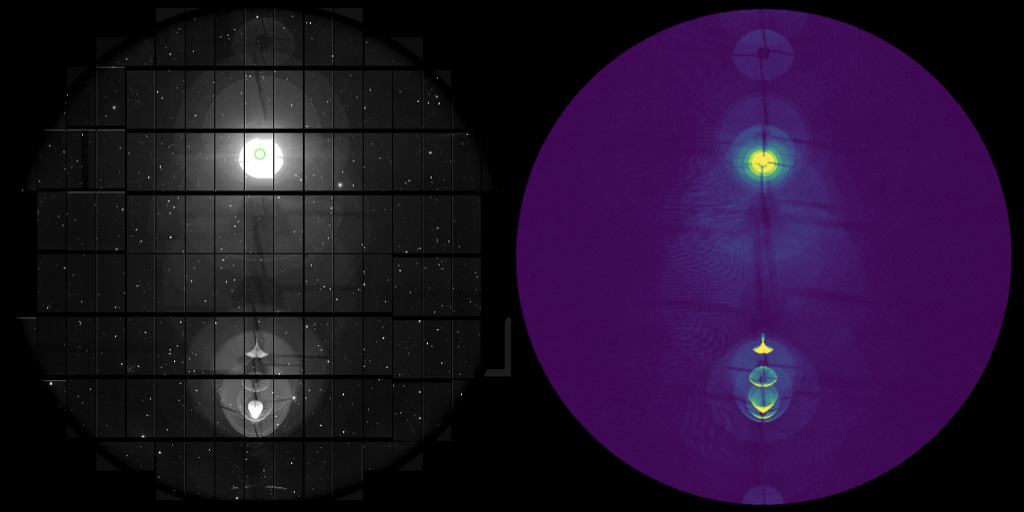
\includegraphics[width=0.9\textwidth]{fig/ghosts_arcturus_crop}
\caption{
Full focal plane HSC image of Arcturus ($0^{\mathrm{th}}$ mag) positioned slightly off axis.
Left: observed HSC data (image credit: Robert Lupton).
Right: reconstructed ghost pattern as predicted using the Batoid software \citep[image credit: ][]{Meyers2019}.
HSC has in-focus ghosts across nearly all the field.
Conversely, Rubin/LSST ghosts will be much farther away from focus as the optics are considerably simpler.
}
\label{fig:ghosts_arcturus_crop}
\end{figure}

We propose a similar on-/off-axis observation exercise with the southern hemisphere star Canopus (V-band magnitude $\sim-0.74$.
In addition to progressive steps off axis, a series of observations with the bright star out of the field of view and at varying rotations is also desirable.
The extreme off-axis angular offset should be chosen based on the observed presence of scattered light artifacts, some of which are undoubtedly unpredictable at present.
Ideally, these data should be taken in good-quality imaging conditions and in dark time where possible.
These data will allow for a focused study of Rubin ghosts, comparing them to the predictions as given by Batoid (see Figure \ref{fig:ghosts_rubin} below for an example prediction).
In particular, the ghosts for Rubin are expected to be much less sharp than those from HSC, which may present obstacles in the LSB regime.

\begin{figure}
\centering
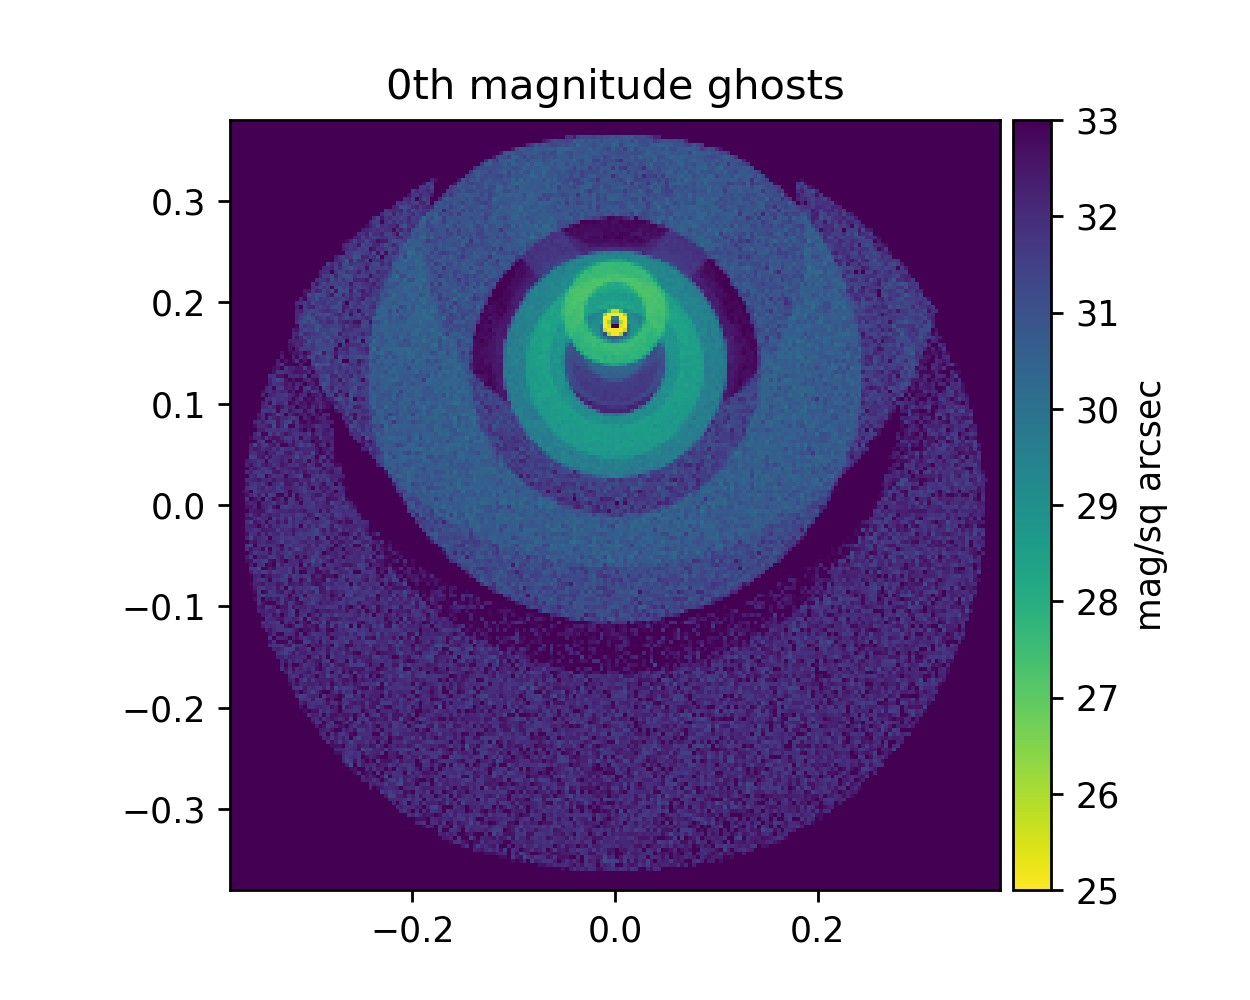
\includegraphics[width=0.75\textwidth]{fig/ghosts_rubin}
\caption{
Ghost surface brightness across the focal plane from a $0^{\mathrm{th}}$ magnitude source placed inside the smallest ghost ring.
Positional x/y units are meters.
Image constructed using Batoid \citep{Meyers2019}, assuming reflection coefficients of 0.02 at every refractive interface except for the filter, which assumes reflection coefficients of 0.5.
Image credit: Josh Meyers.
}
\label{fig:ghosts_rubin}
\end{figure}

In order to detect stray light produced from internal reflections or scattering off of surfaces in the camera and focal plane, we require the following observations.
Most may need $\sim$8 different orientations.
\begin{itemize}
    \item Observations of a bright star located outside of the camera field of view in order to assess grazing incidence reflections off of camera surfaces.
    \item Observations of bright stars located on guider/focus-alignment CCDs to assess the success of the optical model for these CCDs.
    \item Observations of a bright star located in the CCD gaps to test for reflections off of passive surfaces rather than CCDs. 
          It is likely that both both intra-raft and inter-raft CCD gaps will need to be tested.
\end{itemize}

Figure \ref{fig:decam_scattered_light} below shows a low-resolution image of the processed, background-subtracted DECam focal plane taken during Science Verification.
As shown, strong scattering signatures are present, in this case from an off-axis bright star.
Both diffuse ``sprays'' (left) and concentrated (right) features are featured, highlighting some of the potential signatures that may have to be contended with in Rubin operations.

\begin{figure}
\centering
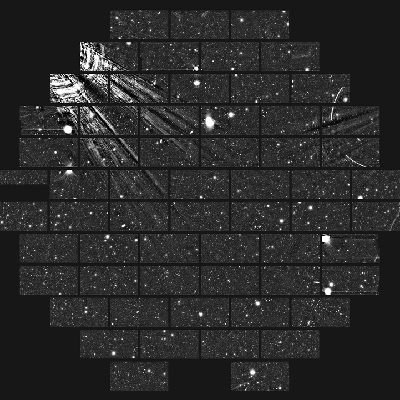
\includegraphics[width=0.55\textwidth]{fig/D00157552_z_r3727p01_sv_400x400.png}
\caption{
Low-resolution image of processed, background-subtracted DECam focal plane taken during Science Verification (exposure number 157552) showing strong signatures of scattered light from an off-axis bright star.
There are both diffuse ``sprays'' (left) and concentrated (right).
See \citet{Kent2013} for a description of the origins of these scattered light feature.
Figure from \citet{Chang2021}.
}
\label{fig:decam_scattered_light}
\end{figure}

% Added by Amir E. Bazkiaei Jul 21
Subtracting bright star wings before estimating the sky background is essential to prevent overestimation of the sky.
To subtract the wings of stars, an extended PSF model of stars is required, usually achieved by stacking normalized stamps of stars.
A parameter that may impact the properties of the extended PSF is the variation with seeing.
To that end, we also request that the telescope be pointed at different altitudes and observations made at different times of the night.

We propose several mosaic observations to provide data for investigating the axial and temporal impacts on the extended PSF. 
For the axial investigation goal, we propose observing a set of five mosaics (patches?) in one night per band.
Each mosaic consists of exposures with pointings at similar altitude.
The altitude of mosaics varies between, and includes, the lowest and the highest possible pointing altitude. 
To have sufficient data to produce the extended PSF, we require each mosaic to consist of at least 10 exposures and each exposure should include at least five stars with a magnitude brighter than 8. 
For the temporal investigation goal, the above should be repeated in multiple nights (maybe four?), and a meaningful time difference between the nights should be considered. 





\subsection{Pinhole camera data}  \label{sec:pinhole}

Initial camera testing will benefit from simple multi-CCD spot projection tools.
The camera team have repurposed one of the initial dummy filters to construct a `pinhole' filter.
This filter is still under development at SLAC but is mostly complete at the time of writing, as shown in Figure \ref{fig:pinhole_lsst}.
A series of 21 pinholes have been drilled into positions corresponding to the center of each raft.
The filter wheel has also been blackened to reduce filter light reflections.

\begin{figure}
\centering
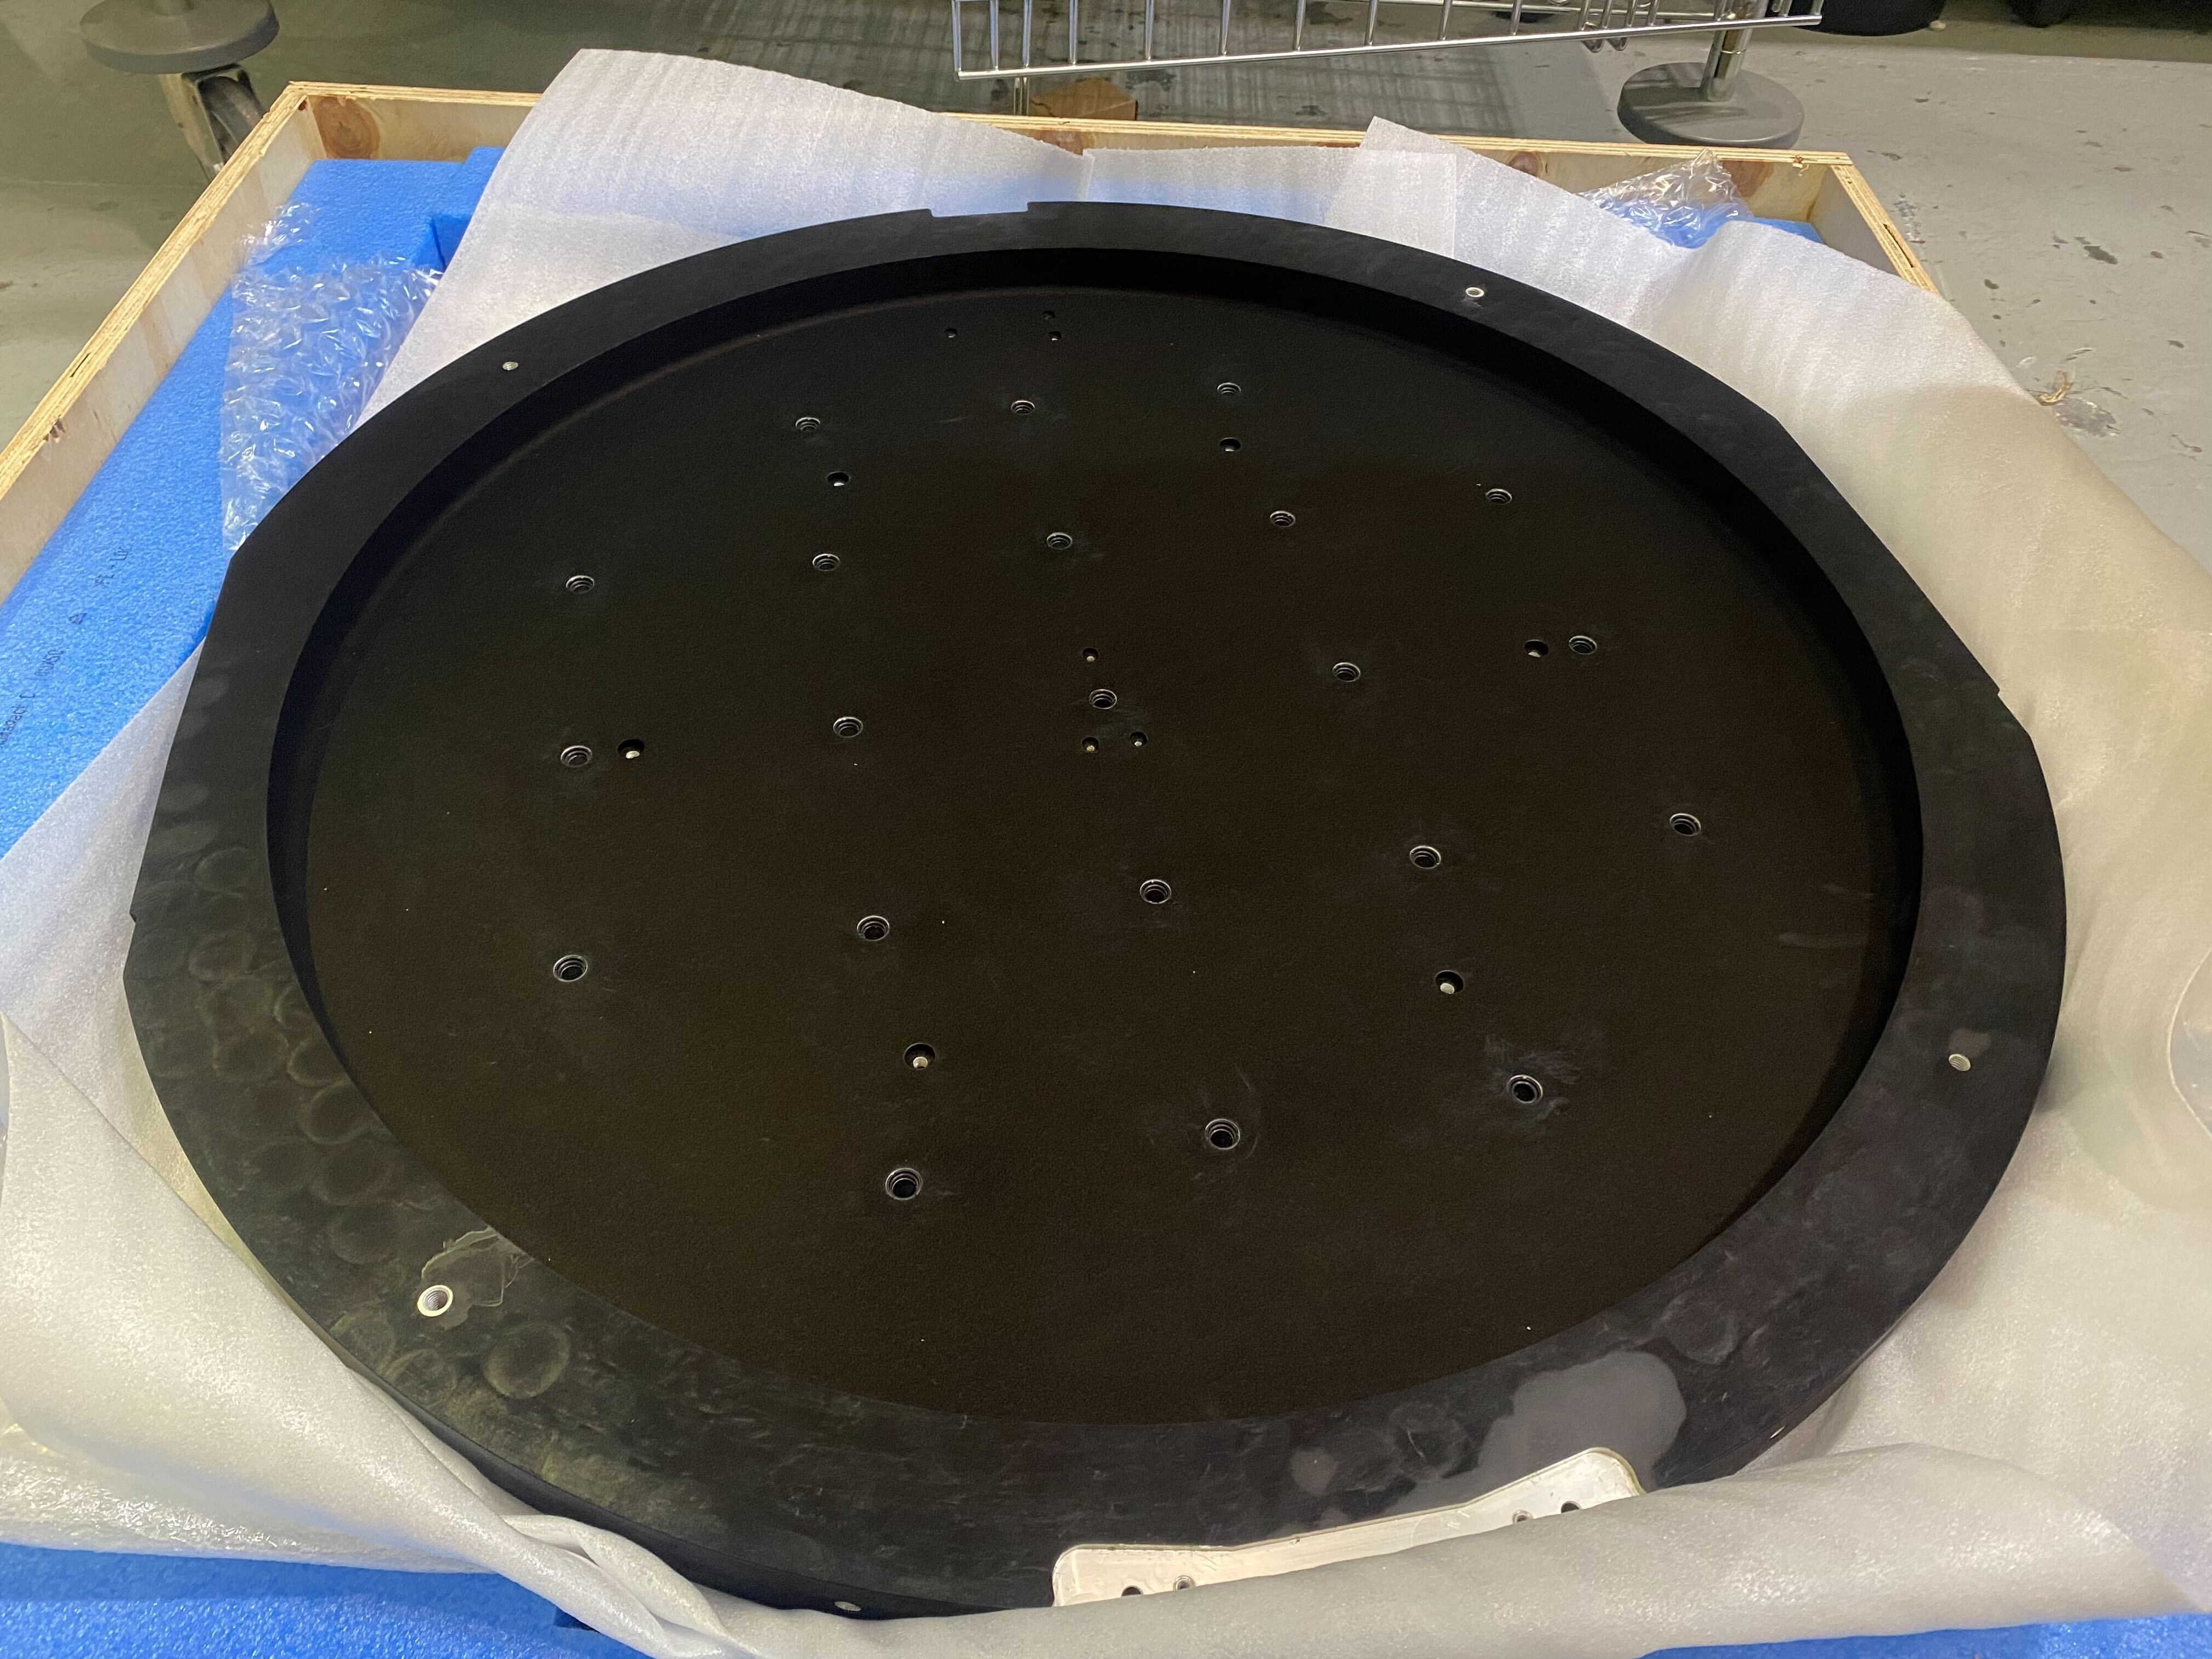
\includegraphics[width=0.75\textwidth]{fig/pinhole_filter_lsst}
\caption{
Pinhole filter for LSST as constructed at SLAC.
A single pinhole has been drilled into a location equivalent to the center of each raft.
Illumination of the instrument with such a filter using a flat field exposure should produce standard stray light/ghost imaging for further analysis.
Image credit: Pierre Antilogus.
}
\label{fig:pinhole_lsst}
\end{figure}

Pinhole data is also useful for studies of stray and scattered light, including ghosting.
Exposure of the optical system with a pinhole filter installed to a dome flat field allows for pristine ghost images to be generated in a controlled environment (21 ghosts, in this case).

Such data has proven useful in earlier studies, for example the HSC team, as shown in Figure \ref{fig:pinhole_hsc}.
In particular, studies of the variation of these pinhole ghosts as a function of position on the focal plane may easily be facilitated via these data.

\begin{figure}
\centering
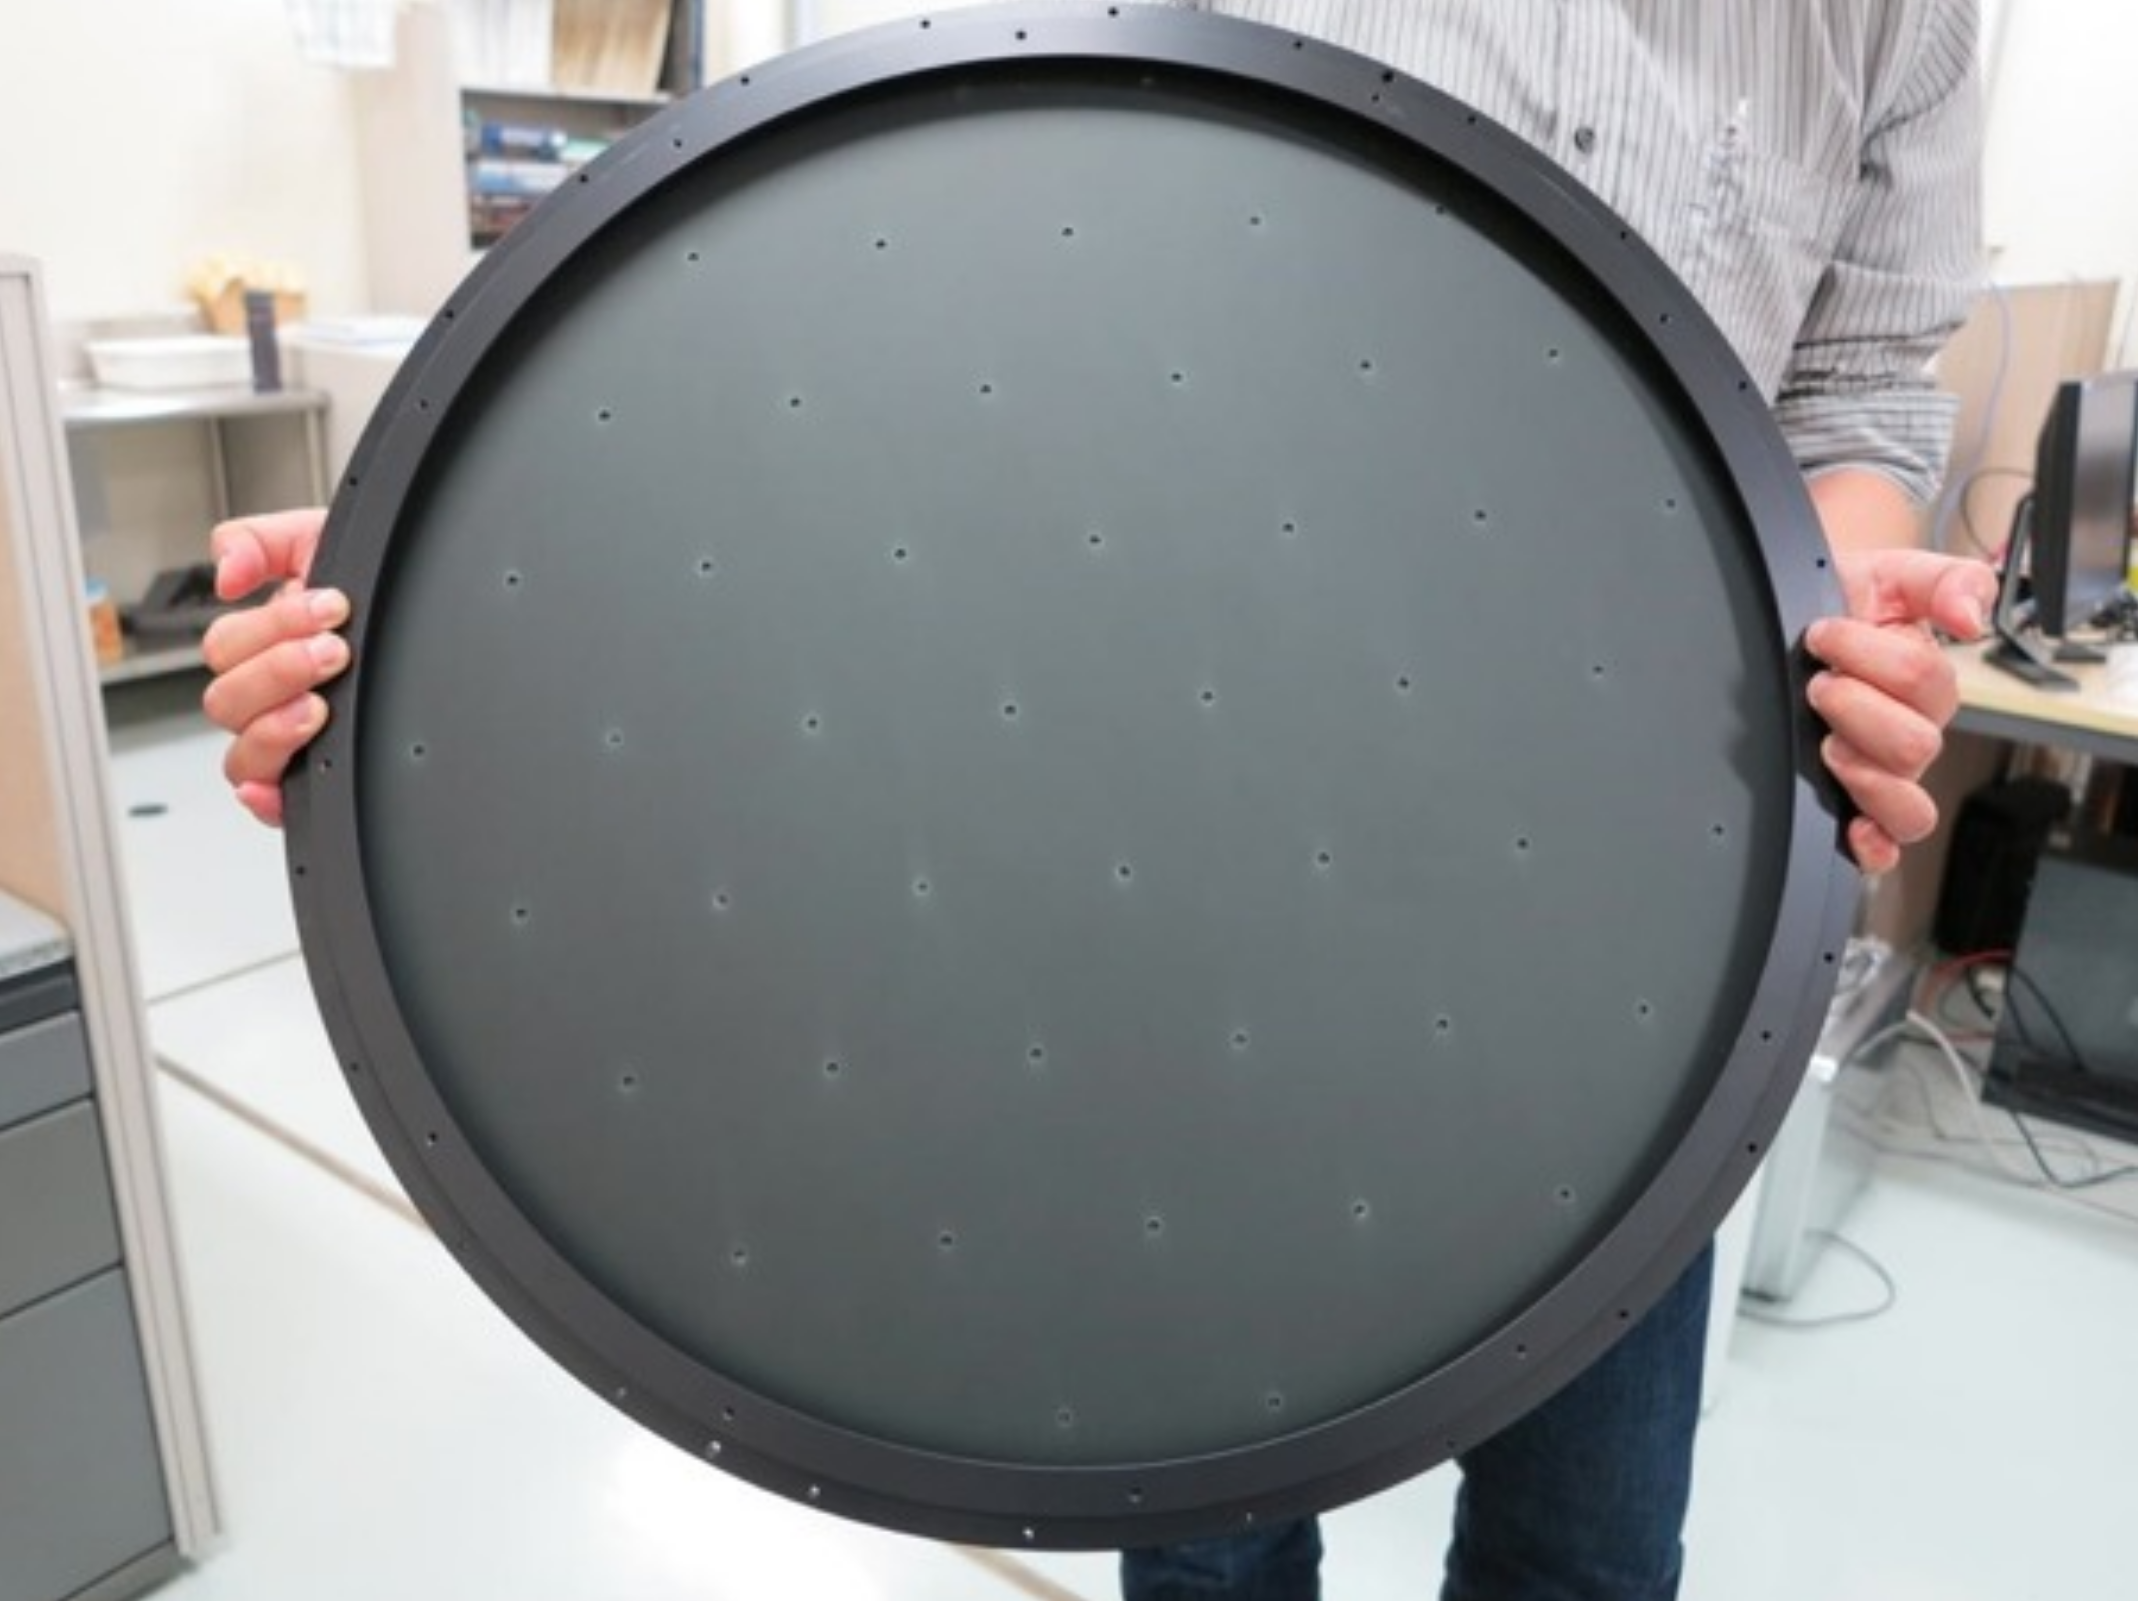
\includegraphics[height=0.4\textwidth]{fig/pinhole_filter_hsc}
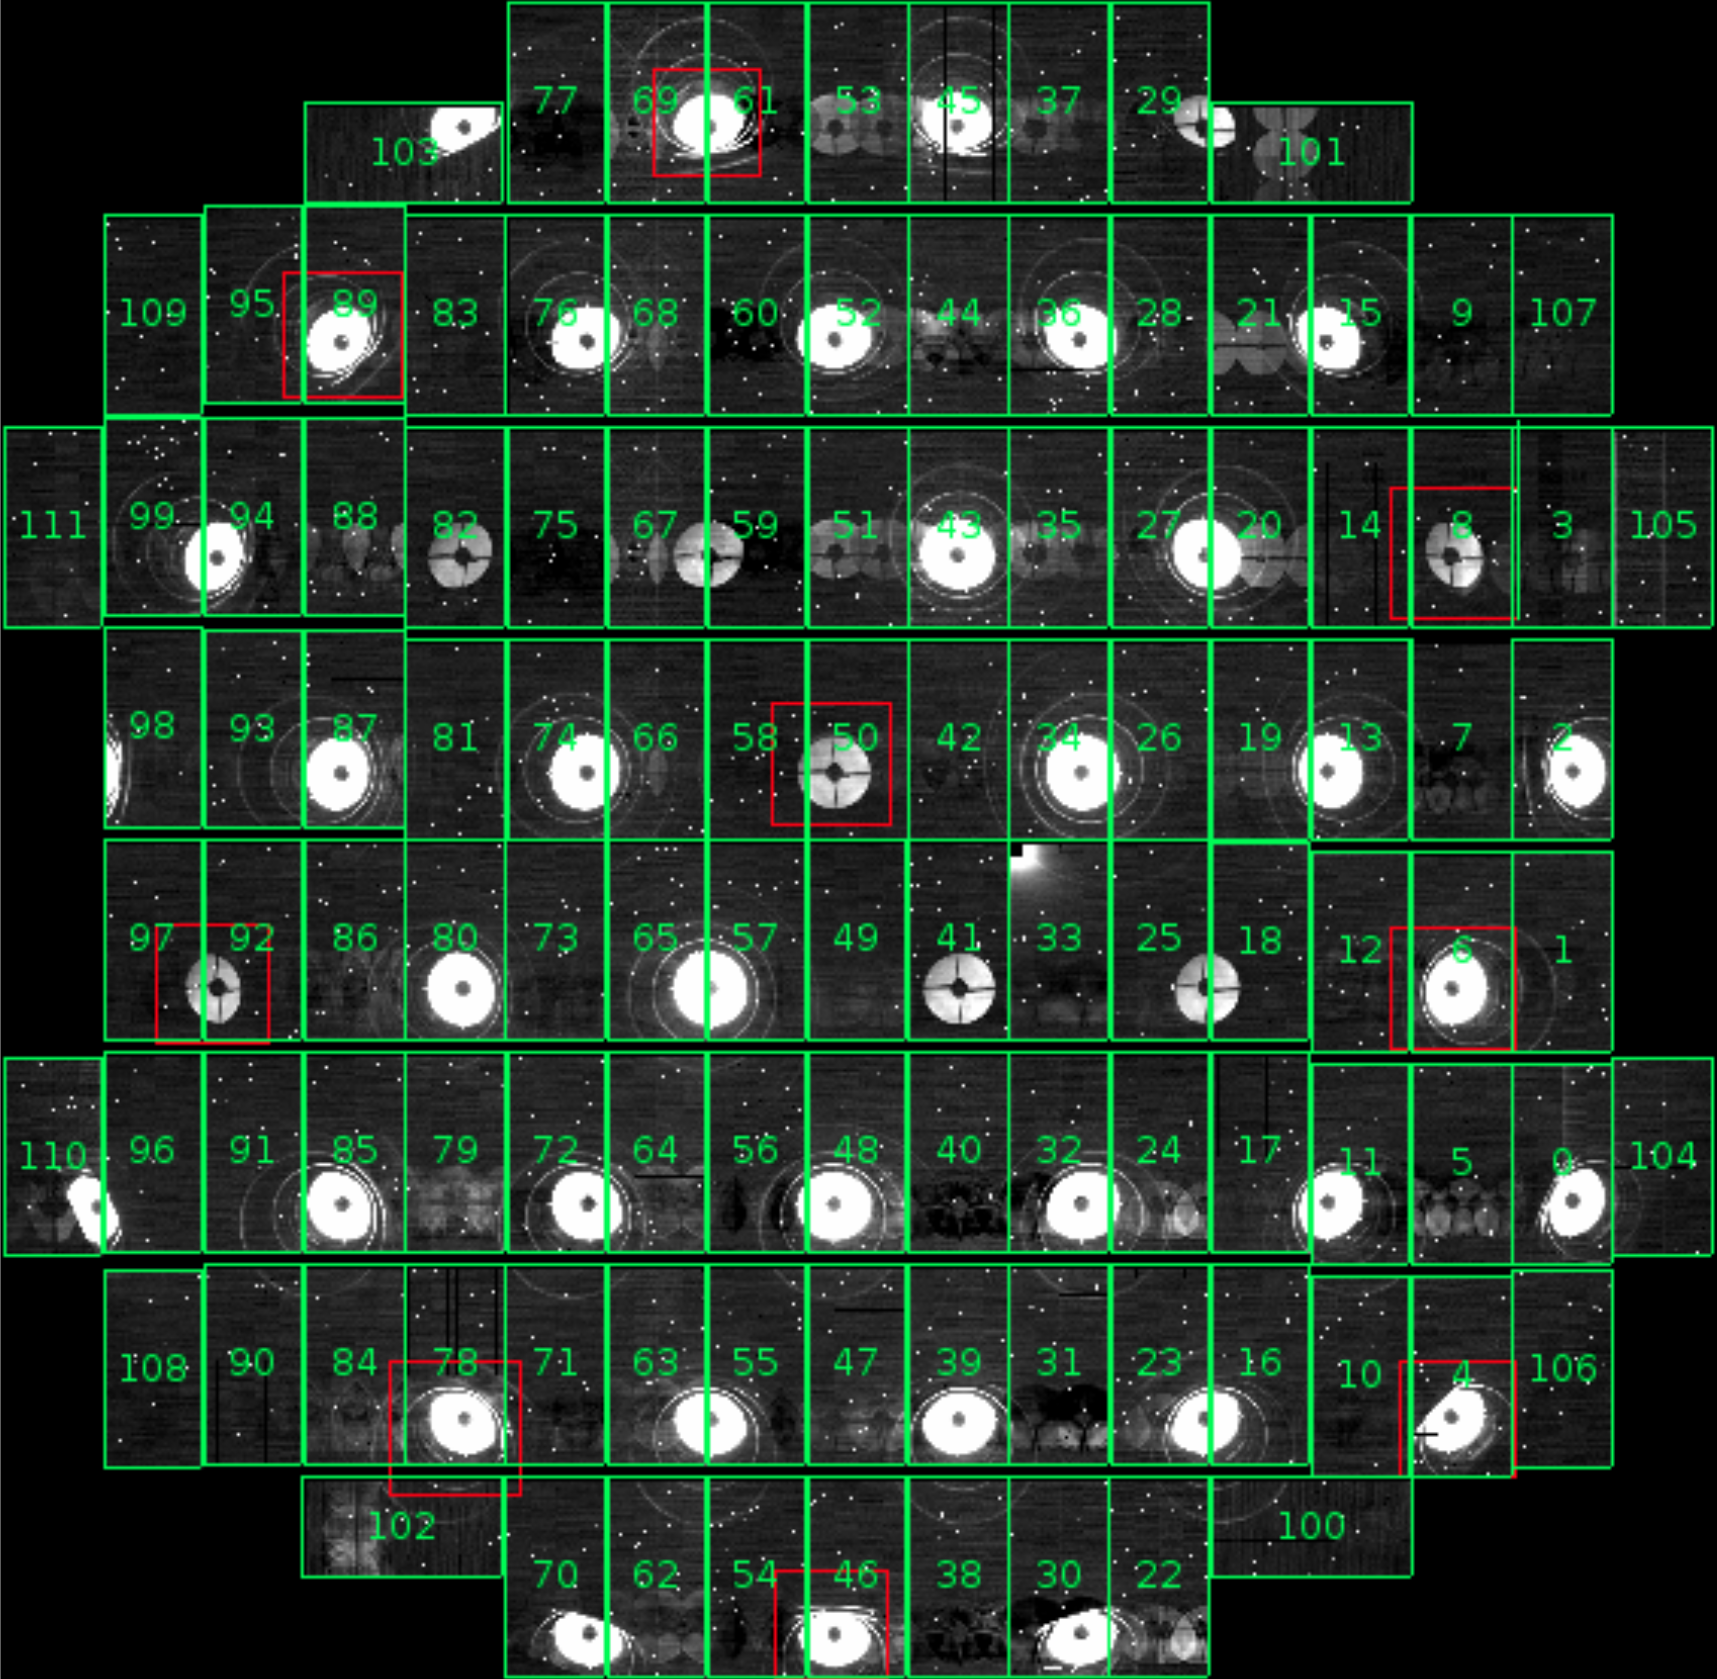
\includegraphics[height=0.4\textwidth]{fig/pinhole_904720}
\caption{
Pinhole filter data for HSC.
Left: Constructed HSC pinhole filter wheel.
Right: Example pinhole data output from the HSC instrument.
Note how exploration of the variation in the ghost as a function of position on the focal plane is possible via these data.
Image credit: Robert Lupton.
}
\label{fig:pinhole_hsc}
\end{figure}

\subsection{Collimated beam projector data}  \label{sec:cbp}

% Edited by Josh on Aug 2
A collimated beam projector (CBP) is a device that produces a beam of light with parallel rays.
Essentially a telescope operated in reverse, a CBP redirects light emitted at the CBP focal plane by a source, such as an LED or laser, to create a beam that does not diverge or converge along its path.

A 25~cm CBP will be installed inside the Rubin dome and used to illuminate individual portions of the Simonyi Survey Telescope primary mirror at a variety of field angles and wavelengths in a controlled manner.
By tracking the relative brightnesses of primary spots and specific ghosts corresponding to specific extra reflections, reflection coefficients as functions of surface, wavelength, position, and incidence angle can be measured.
Gaining access to such data would be very useful in helping us characterize the ghost model and identify unexpected light paths early.

One such example in the recent literature employing this kind of technique is shown in Figure \ref{fig:cbp_pinhole_mondrik2023}, adapted from Figure 5 of \citet{Mondrik2023} \citep[see also][]{Coughlin2016}.
Here, a CBP is operated in conjunction with the StarDICE CCD instrument.
Collimated beams of light are fired into a pinhole filter in order to test and measure transmission at multiple locations across the field of view.
Images are bias corrected and differenced with a dark frame (essentially an exposure taken with the CBP laser shutter closed).\
An enlarged aperture is used to measure the flux throughput at the position of each pinhole source (dark shaded regions), and a local background measure is generated using an outer annulus region (red shaded annuli).
Using these data, the throughput of the StarDICE telescope was able to be measured, indicating a wavelength calibration accuracy of \sim 0.1 nm.

\begin{figure}
\centering
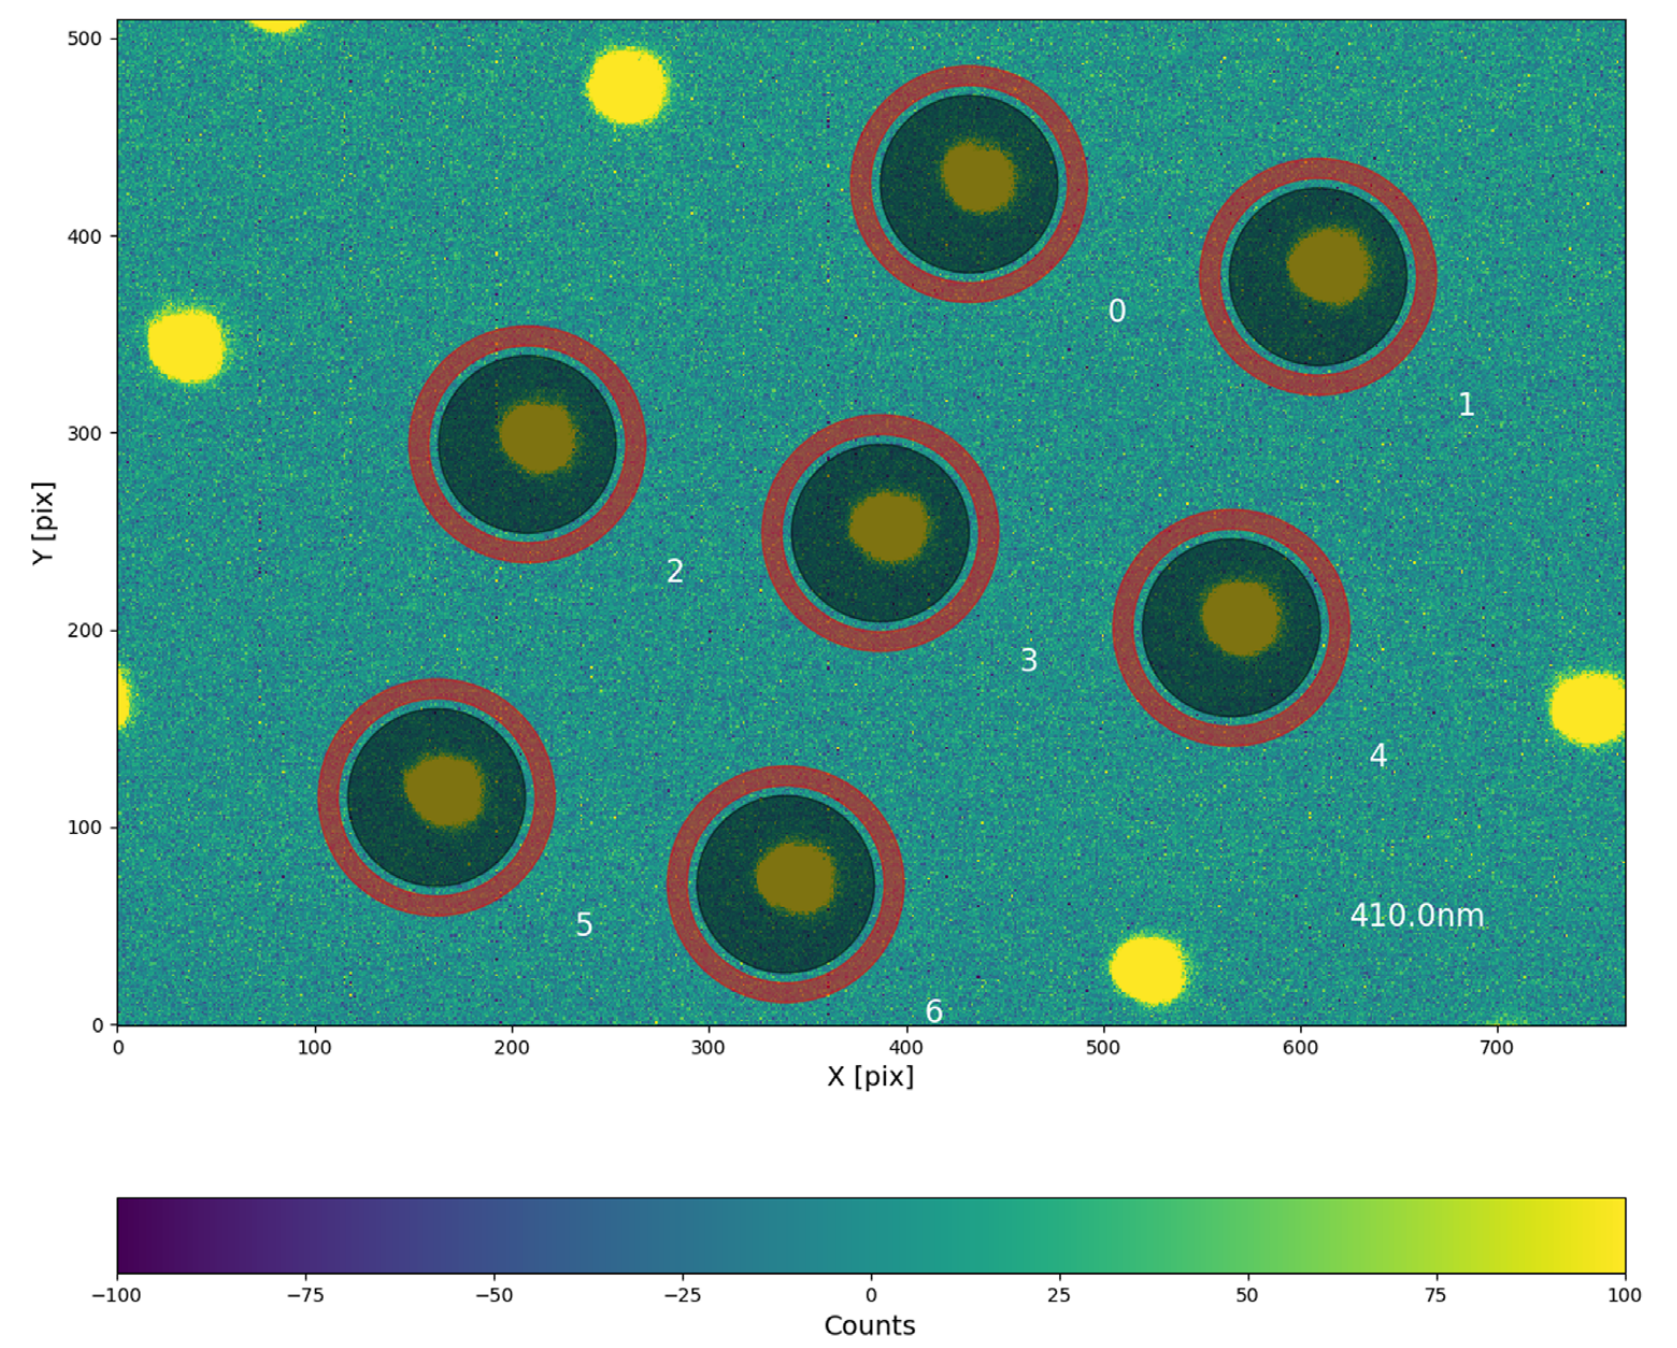
\includegraphics[height=0.75\textwidth]{fig/cbp_pinhole_mondrik2023}
\caption{
An image of the 5 × 5 20 μm pinhole mask as seen by the StarDICE CCD.
In this experiment, CBP light is passed through a pinhole filter to test transmission at different locations across the detector.
Black shaded regions are used to calculate aperture photometry for each source, and red annuli are used to generate local background estimates at the position of each source.
Note the minor aberrations in the pinhole shapes, caused by the beam being slightly out of collimation.
Figure adapted from Figure 5, \citet{Mondrik2023}.
}
\label{fig:cbp_pinhole_mondrik2023}
\end{figure}





\subsection{Full moon data}  \label{sec:fullmoon}

During full moon, a grid of observations with the Moon at different angular positions from the array should be taken.
Minimally, this should include a series of short exposures spaced 5 degrees apart (closer if possible) starting with the Moon 45 degrees NW and ending with the Moon 45 degrees SE of the main array (skipping the ones where the Moon will be on the array) to check for ghouls related to the Moon.

This might be acquired over multiple nights, as the key offset is between the full Moon and the detector array, but there is a small concern that non-moving parts of the observatory might also be involved in scattering moonlight into the beam.
This may require a repeat of the observations with the Moon in a different orientation relative to the observatory.
Due to the relatively large angular size of the moon, image quality is not a limiting factor for these observations.





%Added by Yao on Jul 10
\subsection{Galactic Cirrus}  \label{sec:cirrus}

We should aim to observe a few patches of sky with different levels of Galactic cirrus coverage/intensity.
Galactic cirrus can significantly affect sky brightness determination and photometric measurement \citep[see, e.g., ][]{Jeong2005, Roman2020}.
The range of Galactic cirrus coverage can be used to determine how severe those impacts are.
Higher quality imaging would be preferable here, as our ability do distinguish and deblend cirri from their other surrounding astrophysical sources may be a limiting factor.
However, if observations of galactic cirrus are performed in less-than-ideal observing conditions (e.g., as part of other observing campaigns), these data may also prove useful here, allowing us to test and better understand how cirri impact sky subtraction and photometric performance in lower quality imaging.





\newpage

\appendix
% Include all the relevant bib files.
% https://lsst-texmf.lsst.io/lsstdoc.html#bibliographies
\section{References} \label{sec:bib}
\renewcommand{\refname}{} % Suppress default Bibliography section
\bibliography{local,lsst,lsst-dm,refs_ads,refs,books}

% Make sure lsst-texmf/bin/generateAcronyms.py is in your path
\section{Acronyms} \label{sec:acronyms}
\addtocounter{table}{-1}
\begin{longtable}{p{0.145\textwidth}p{0.8\textwidth}}\hline
\textbf{Acronym} & \textbf{Description}  \\\hline

DM & Data Management \\\hline
\end{longtable}

% If you want glossary uncomment below -- comment out the two lines above
%\printglossaries





\end{document}
